\documentclass[preprint,12pt]{elsarticle}

%% Use the option review to obtain double line spacing
%% \documentclass[preprint,review,12pt]{elsarticle}

%% Use the options 1p,twocolumn; 3p; 3p,twocolumn; 5p; or 5p,twocolumn
%% for a journal layout:
%% \documentclass[final,1p,times]{elsarticle}
%% \documentclass[final,1p,times,twocolumn]{elsarticle}
%% \documentclass[final,3p,times]{elsarticle}
%% \documentclass[final,3p,times,twocolumn]{elsarticle}
%% \documentclass[final,5p,times]{elsarticle}
%% \documentclass[final,5p,times,twocolumn]{elsarticle}

%% The graphicx package provides the includegraphics command.
\usepackage[margin=1in]{geometry}
\usepackage{graphicx}
%% The amssymb package provides various useful mathematical symbols
\usepackage{amssymb}
%% The amsthm package provides extended theorem environments
\usepackage{amsthm}
\usepackage{amsmath}
\usepackage{setspace}
\usepackage{lscape}
\usepackage{booktabs}
\usepackage[scr]{rsfso}
\usepackage{xcolor}
\usepackage{soul}

%% The lineno packages adds line numbers. Start line numbering with
%% \begin{linenumbers}, end it with \end{linenumbers}. Or switch it on
%% for the whole article with \linenumbers after \end{frontmatter}.
\usepackage{lineno}
\DeclareMathOperator*{\argminA}{arg\,min}
\DeclareMathOperator*{\argmaxA}{arg\,max}
\newtheorem{defn}{Definition}

%% natbib.sty is loaded by default. However, natbib options can be
%% provided with \biboptions{...} command. Following options are
%% valid:

%%   round  -  round parentheses are used (default)
%%   square -  square brackets are used   [option]
%%   curly  -  curly braces are used      {option}
%%   angle  -  angle brackets are used    <option>
%%   semicolon  -  multiple citations separated by semi-colon
%%   colon  - same as semicolon, an earlier confusion
%%   comma  -  separated by comma
%%   numbers-  selects numerical citations
%%   super  -  numerical citations as superscripts
%%   sort   -  sorts multiple citations according to order in ref. list
%%   sort&compress   -  like sort, but also compresses numerical citations
%%   compress - compresses without sorting
%%
%% \biboptions{comma,round}

% \biboptions{}

%%% Change the date
\newcommand{\mathcolorbox}[2]{\colorbox{#1}{$\displaystyle #2$}}
\renewcommand*{\today}{Dec. 18, 2023}

\journal{Dr. Choi \& Dr. Espin-Garcia}

\begin{document}

\begin{frontmatter}

%% Title, authors and addresses

\title{Jiaqi's Thesis Progress Report (Updated Dec. 18)}


%% use optional labels to link authors explicitly to addresses:
%% \author[label1,label2]{}
%% \address[label1]{}
%% \address[label2]{}


\author[rvt]{Jiaqi Bi}
\ead{jbi23@uwo.ca}
%\author[rvt]{Jiaqi Bi\corref{cor1}\fnref{fn1}}
%\ead{jbi23@uwo.ca}
%\author[rvt]{E.~Deccache\fnref{fn1}}
%\ead{elciodeccache@unifei.edu.br }
%\author[rvt]{B.D.~Bonatto\fnref{fn1}}
%\ead{bonatto@unifei.edu.br }
%\author[rvt]{H.~Arango\fnref{fn1}}
%\ead{hector.arango@uol.com.br }
%\author[rvt]{E.O.~Pamplona\fnref{fn2}}
%\ead{pamplona@unifei.edu.br}
%%\author[els]{E.O.~Pamplona\corref{cor2}\fnref{fn1,fn3}}
%%\ead[url]{pamplona@unifei.edu.br}
%%\cortext[cor1]{Corresponding author}
%\cortext[cor2]{Affliated with Schulich School of Medicine \& Dentistry, Dept. Epidemiology and Biostatistics}
%\fntext[fn1]{Study Affiliated with Department of Statistical and Actuarial Sciences}
%\cortext[cor2]{Principal corresponding author}
%\fntext[fn1]{CERIn - Center of Excellence in Smart Grids}
%\fntext[fn2]{IEPG - Management \& Production Engineering Institute \\Unifei - Federal University of Itajuba}

\address[rvt]{Western University, \\ Schulich School of Medicine \& Dentistry, \\ Department of Epidemiology and Biostatistics}

%\tnotetext[t1]{The authors would like to thank ELETROBRAS, ANEEL, INERGE, CAPES, CNPq and FAPEMIG for financially supporting this research.}

%% use the tnoteref command within \title for footnotes;
%% use the tnotetext command for the associated footnote;
%% use the fnref command within \author or \address for footnotes;
%% use the fntext command for the associated footnote;
%% use the corref command within \author for corresponding author footnotes;
%% use the cortext command for the associated footnote;
%% use the ead command for the email address,
%% and the form \ead[url] for the home page:
%%
%% \title{Title\tnoteref{label1}}
%% \tnotetext[label1]{}
%% \author{Name\corref{cor1}\fnref{label2}}
%% \ead{email address}
%% \ead[url]{home page}
%% \fntext[label2]{}
%% \cortext[cor1]{}
%% \address{Address\fnref{label3}}
%% \fntext[label3]{}


%% use optional labels to link authors explicitly to addresses:
%% \author[label1,label2]{<author name>}
%% \address[label1]{<address>}
%% \address[label2]{<address>}

%\begin{abstract}
%\setstretch{1.2}
%% Text of abstract

%\end{abstract}

%\begin{keyword}
%Electricity theft \sep Regulated Electricity Company \sep Economic Impact \sep Tarot \sep Operational Optimal Point.
%% keywords here, in the form: keyword \sep keyword
%Missing data \sep Multiple imputation \sep complete case analysis \sep EM algorithm \sep MCMC
%% MSC codes here, in the form: \MSC code \sep code
%% or \MSC[2008] code \sep code (2000 is the default)

%\end{keyword}

\end{frontmatter}

%%
%% Start line numbering here if you want
%%
\linenumbers
%\setstretch{1.5}
%% main text
\section{To Do List during the Christmas}
\begin{enumerate}
    \item Correlated frailty - NR-algorithm
    \item Using importance weights to implement MCEM
    \item Multiple imputation - similar imputation step as MCEM
\end{enumerate}
\section{Weibull Parametric Approach and MCEM Method}
From the beginning of the discussion, I have obtained the model, i.e., the hazard function is
\begin{equation}
    h_{ij}(t_{ij}|z_j)=h_0(t_{ij})\exp(\beta_1g_{ij}+\beta_2 x_{ij})z_j
\end{equation}
where $g_{ij}$ is the genotype, or say mutation gene status for individual $i$ in family $j$, and $x_{ij}$
is the PRS for individual $i$ in family $j$. The frailty term $z_j$, has a pdf of $f(z)$, which can be Gamma, or log-normal, 
to ensure the support is always non-negative. The Weibull baseline hazard function is defined as
\begin{equation}
    h_0(t_{ij})=\alpha\lambda t_{ij}^{\lambda-1}
\end{equation}
where $\lambda$ is the shape parameter and $\alpha$ is the scale parameter. Let $\xi_{ij}=\exp(\beta_1 g_{ij}+\beta_2 x_{ij})$, the hazard function is 
\begin{equation}
    h_{ij}(t_{ij}|x_{ij}, g_{ij}, z_j)=\alpha\lambda t_{ij}^{\lambda-1}\xi_{ij}z_j
\end{equation}
The survival function $S(t)$ can be obtained through cumulative hazard function $H(t)$
\begin{align}
    H(t_{ij}|x_{ij}, g_{ij}, z_j)&=\int_0^{t}h_{ij}(u|\cdot)du\\
    &=\alpha\xi_{ij}z_j\lambda\int_0^t u^{\lambda-1}du\\
    &=\alpha\xi_{ij}z_j\lambda\cdot \frac{1}{\lambda} t_{ij}^{\lambda}=\alpha\xi_{ij}z_j t_{ij}^{\lambda}
\end{align}
and the survival function
\begin{equation}
    S(t_{ij}|x_{ij}, g_{ij}, z_j)=\exp(-H(t_{ij}|\cdot))=\exp(-\alpha\xi_{ij}z_j t_{ij}^{\lambda})
\end{equation}
Therefore, the likelihood can be written as
\begin{align}
    L(\beta_1, \beta_2, \lambda, \alpha; x_{ij}, g_{ij}, t_{ij}, \delta_{ij}, z_j)=\prod_{j=1}^k\int_0^{\infty}\prod_{i=1}^{n}(\alpha\lambda t_{ij}^{\lambda-1}\xi_{ij}z_j)^{\delta_{ij}}\exp(-\alpha\xi_{ij}z_j t_{ij}^{\lambda})f(z)dz
\end{align}
So the log-likelihood is 
\begin{equation}\label{eq:logllhd}
    \ell(\beta_1, \beta_2, \lambda, \alpha; x_{ij}, g_{ij}, t_{ij}, \delta_{ij}, z_j)=\sum_{j=1}^k\log \left [ \int_0^{\infty}\prod_{i=1}^{n_j}(h(t_{ij}|\mathbf{x}_{ij}, z_j))^{\delta_{ij}}\exp (-H(t_{ij}|\mathbf{x}_{ij}, z_j))f(z_j)dz_j\right ]
\end{equation}

\section{Gamma Frailty} 
The Laplace transform of the frailty $f(z_j)=\text{Gamma}(v_j, v_j)$, for the simplicity of the mathematical expression, the following Laplace transform will ignore the subscript, denote $\mathscr{L}(f(z))=\phi(\cdot)$:
\begin{align}
    \mathscr{L}(f(z))=\phi(s)&=\int_0^{\infty}e^{-sz}f(z)dz\\
    &=\int_0^{\infty}e^{-sz}\frac{v^v}{\Gamma(v)}z^{v-1}e^{-vz}dz
\end{align}
Using the Gamma property: $\int_0^{\infty}z^{n-1}e^{-az}dz=\frac{\Gamma(n)}{a^n}$, $\phi(s)$ can be further written as
\begin{equation}
    \phi(s)=\frac{v^v}{\Gamma(v)}\int_0^{\infty}e^{-(s+v)z}z^{v-1}dz=\frac{v^v}{\Gamma(v)}\cdot \frac{\Gamma(v)}{(s+v)^v}=(1+\frac{s}{v})^{-v}
\end{equation}
The second derivative is $\frac{d^2\phi(s)}{ds^2}=\int_0^{\infty}(-z)^2e^{-sz}f(z)dz$. 

\noindent
The third derivative is $\frac{d^3\phi(s)}{ds^3}=\int_0^{\infty}(-z)^3e^{-sz}f(z)dz$, ...
Therefore, its $d$-th derivative, denote $\phi(s)^{(d)}$:
\begin{align}
    \phi(s)^{(d)}&=(-1)^d\int_0^{\infty}z^de^{-sz}f(z)dz\\
    &=(-1)^d\frac{(v+d-1)!}{(v-1)!(s+v)^d}(1+\frac{s}{v})^{-v}
\end{align}
for some function $s$ that does not involve with $z$. Let $\boldsymbol{\theta}=(\beta_1, \beta_2, \alpha, \lambda)$, the log-likelihood is then written as
\begin{align}
    \ell(\boldsymbol{\theta})&=\sum_{j=1}^k\log \left [ \int_0^{\infty}\prod_{i=1}^{n_j}(h(t_{ij}|\mathbf{x}_{ij}, z_j))^{\delta_{ij}}\exp (-H(t_{ij}|\mathbf{x}_{ij}, z_j))f(z_j)dz_j\right ]\\
    &=\sum_{j=1}^k\log\left [\int_{0}^{\infty}\prod_{i=1}^{n_j}(z_j h(t_{ij}|\mathbf{x}_{ij}))^{\delta_{ij}}\exp(-z_j H(t_{ij}|\mathbf{x}_{ij}))f(z_j)dz_j\right ]\\
    &=\sum_{j=1}^k\log\left [\prod_{i=1}^{n_j}(h(t_{ij}|\mathbf{x}_{ij}))^{\delta_{ij}}\int_0^{\infty}z_j^{d_j}\exp(-z_j\sum_{i=1}^{n_j}H(t_{ij}|\mathbf{x}_{ij}))f(z_j)dz_j \right ]\\
    &=\sum_{j=1}^k\log\left [\prod_{i=1}^{n_j}(h(t_{ij}|\mathbf{x}_{ij}))^{\delta_{ij}}\frac{(v+d_j-1)!}{(v-1)!(\sum_{i=1}^{n_j}H(t_{ij}|\mathbf{x}_{ij})+v)^{d_j}}\Big(1+\frac{\sum_{i=1}^{n_j}H(t_{ij}|\mathbf{x}_{ij})}{v}\Big)^{-v}\right ]\\
    &=\sum_{j=1}^k\log\left [\prod_{i=1}^{n_j}((h(t_{ij}|\mathbf{x}_{ij}) )^{\delta_{ij}})\frac{(v+d_j-1)!}{v!v^{d_j-1}}(1+\frac{\sum_{i=1}^{n_j}(H(t_{ij}|\mathbf{x}_{ij}))}{v})^{-v-d_j} \right ]\\
    &=\sum_{j=1}^k\log\left [(h(\cdot))^{\delta_{ij}} \frac{(v+d_j-1)!}{v!v^{d_j-1}}(1+\frac{\sum_{i=1}^{n_j}(H(t_{ij}|\mathbf{x}_{ij}))}{v})^{-v-d_j} \right ]\\
    &=\sum_{j=1}^k\left [\sum_i(\delta_{ij}\log h(\cdot)) + \log\Big (\frac{(v+d_j-1)!}{v!v^{d_j-1}}(1+\frac{\sum_{i=1}^{n_j}(H(t_{ij}|\mathbf{x}_{ij}))}{v})^{-v-d_j}\Big )\right ]
\end{align}
For each family $j$, the ascertainment is defined to be the probability of the proband $p$ being ascertained by the age $a_{j_p}$ at examination, denoting $A_j$. Applying the ascertainment correction for the log-likelihood in family $j$: 
\begin{equation}
    \ell(\cdot)=\ell_j(\cdot)-\log A_j(\cdot)
\end{equation}
note we can still apply Laplace transform here, such that
\begin{align}
    A_j(\cdot)&=1-S_{j_p}(a_{j_p}|X_{j_p})\\
    &=1-\int_Z S_{j_p}(a_{j_p}|X_{j_p},z_j)f(z_j)dz_j\\
    &=1-\int_Z\exp(-z_j\cdot H_{j_p}(a_{j_p}|X_{j_p}))f(z_j)dz_j\\
    &=1-(1+\frac{H_{j_p}(a_{j_p}|X_{j_p})}{k})^{-k}
\end{align}
\section{Log-Normal Frailty}
The log-normal frailty is not the power-variance-function (PVF) family, so there is no closed form for Laplace transform or expressions for survivors. But we are able to estimate the Laplace transform using Gauss Hermite Quadrature. We typically standardize the log-normal frailty $Z$ as
\begin{align} 
    E(\log Z)&=0\\
    \text{Var}(\log Z)&=\sigma^2
\end{align} 
That is, $Z_j\sim \text{log-Normal}(0, \sigma^2)$. The probability density function $f(z_j)$ is then
\begin{equation}\label{eq:lognormalfrailty}
    f(z_j)=\frac{1}{\sqrt{2\pi}\sigma}z_j^{-1}\exp (-\frac{\log (z_j)^2}{2\sigma^2})
\end{equation}
The Laplace transform is then
\begin{equation}
    \phi(s)=\mathscr{L}(f_Z)(s)=\int_0^{\infty}\exp(-sz)\cdot f(z)dz
\end{equation}
Using variable transformation, let $y=\frac{\log(z)}{\sqrt{2}\sigma}$, then $z=\exp(\sqrt{2}\sigma y)$, and $dz=\sqrt{2}\sigma\exp(\sqrt{2}\sigma y)dy$. Therefore, for $d$-th derivative:
\begin{align}
    \phi(s)^d&=\int_{-\infty}^{\infty}z^d\exp(-sz)\cdot\frac{1}{\exp(\sqrt{2}\sigma y)\sigma\sqrt{2\pi}}\cdot\exp(-y^2)\cdot\sqrt{2}\sigma\exp(\sqrt{2}\sigma y)dy\\
    &=\int_{-\infty}^{\infty}\exp(\sqrt{2}\sigma y)^d\exp(-s\exp(\sqrt{2}\sigma y))\cdot\frac{1}{\sqrt{\pi}}\exp(-y^2)dy
\end{align}
\begin{defn}[Gauss-Hermite Quadrature]\label{defn:gausshermite}
    The integrand part can be solved using Gauss-Hermite Quadrature. In numerical analysis, the method can be applied in the following form:
\begin{equation}
    \int_{-\infty}^{\infty}\exp(-x^2)f(x)dx\approx \sum_{i=1}^n\omega_i f(x_i)
\end{equation}
where $n$ is number of sample points used, and $x_i$ is the roots of Hermite polnomial $H_n (x)$ such that $i=1, ..., n$, and the weights $\omega_i$ is 
\begin{equation}
    \omega_i=\frac{2^{n-1}n!\sqrt{n}}{n^2[H_{n-1}(x_i)]^2}
\end{equation}
\end{defn}

\noindent
Applying Definition~\ref{defn:gausshermite}, the integral of the Laplace transform is then
\begin{equation}
    \phi(s)^d=\frac{1}{\sqrt{\pi}}\sum_{p=1}^{N_p}\omega_p\exp(-s\exp(\sqrt{2}\sigma y_p))\exp(\sqrt{2}\sigma y_p)^d
\end{equation}
Thus, substituting into the log-likelihood:
\begin{equation}
    \ell_j(\cdot)=\sum_{i=1}^{n_j}\delta_{ij}\log(h(t_{ij}|\mathbf{x}_{ij}))+\log\Big (\frac{1}{\sqrt{\pi}}\sum_{p=1}^{N_p}\left [\omega_p\exp(\sqrt{2}\sigma y_p)^{d_{ij}}\exp\Big (-\sum_{i=1}^{n_j}H(t_{ij}|\mathbf{x}_{ij})\exp(\sqrt{2}\sigma y_p)\Big )\right ]\Big )
\end{equation}
Similarly, the ascertainment correction in the log-normal frailty can be written as 
\begin{align}
    A_j(\cdot)&=1-\int_Z \exp(-z_j H_{j,p}(a_{j,p}|\mathbf{x}_{j,p}))f(z_j)dz_j\\
    &=1-\sum_{p=1}^{N_p}\omega_p \exp\left (-(\sum_{i=1}^{n_j} H(a_{j,p}|\mathbf{x}_{ij}))\exp (\sqrt{2}\sigma y_{p})\right )
\end{align}

\section{Correlated Frailty using Kinship Matrix}
Family members are correlated within one family, that we denote $K$ as the kinship correlation matrix among all observations. This matrix ensures those individuals not from the same family automatically have a correlation of 0. The likelihood construction needs multivariate form. For $\mathbf{Z}\sim\text{MVN}(0,\sigma^2K)$, that $K$ has the diagonal of 1. The likelihood is 

\begin{align}
    L(\cdot)&=\int_{\mathbb{R}^n}\prod_{i=1}^n(h(t|\mathbf{x}_i, \mathbf{z}_i))^{\delta_i}\exp (-H(t|\mathbf{x}_i, \mathbf{z}_i))f(\mathbf{z})d\mathbf{z}\\
    &=\int_{\mathbb{R}^n}\prod_{i=1}^n(h(t|\mathbf{x}_i))^{\delta_i}\exp(\mathbf{z}_i)^{\delta_i}\exp(-H(t|\mathbf{x}_i)\exp(\mathbf{z}_i))f(\mathbf{z})d\mathbf{z}\\
    &=\prod_{i=1}^n(h(t|\mathbf{x}_i))^{\delta_i}\int_{\mathbb{R}^n}\exp(\delta_i\mathbf{z}_i-H(t|\mathbf{x}_i)\exp(\mathbf{z}_i))f(\mathbf{z})d\mathbf{z}
\end{align}
Applying the Laplace approximation, and taking the log for the likelihood, we obtain
\begin{equation}
    \ell(\cdot)=\sum_{i=1}^n\Big [ \delta_i\log h(t|\mathbf{x}_i)\Big ] + \sum_{i=1}^n\Big [\delta_i \hat{\mathbf{z}}-H(t_i|\mathbf{x}_i)\exp(\hat{\mathbf{z}})\Big ] - \frac{1}{2}\hat{\mathbf{z}}^{\top}\Sigma^{-1}\hat{\mathbf{z}}
\end{equation}
such that $\Sigma=\sigma^2 K$. Also, we treat the random effect $\mathbf{z}$ as a vector of parameters, and use outer-loop to search for the $\sigma$, and use inner-loop to search for other parameters (baseline parameters, and $\beta$) including $\mathbf{z}$. The process can be achieved via Newton-Raphson algorithm. For computational efficiency, we can set $\Sigma^{-1}=L^{\top}L$ through Cholesky Decomposition. In this way, 
$\mathbf{z}L\sim MVN(0,\sigma^2 I)$. In order to apply NR-algorithm, the gradient and the hessian are required. The gradient for parameters is:
\begin{equation}
    \frac{\partial\ell}{\partial\boldsymbol{\beta}}=\sum_{i=1}^n\delta_i\mathbf{x}_i+\sum_{i=1}^n-H(t_i|\mathbf{x}_i)\mathbf{x}_i\exp(\mathbf{z})
\end{equation}

\begin{equation}
    \frac{\partial\ell}{\partial\mathbf{z}}=\sum_{i=1}^n\delta_i-(t_i|\mathbf{x}_i)\exp(\hat{\mathbf{z}})-\Sigma^{-1}\hat{\mathbf{z}}
\end{equation}

\begin{equation}
    \frac{\partial\ell}{\partial\alpha}=\sum_{i=1}^n\frac{\delta_i}{\alpha} + \sum_{i=1}^n-\frac{H(t_i|\mathbf{x}_i)\exp(\hat{\mathbf{z}})}{\alpha}
\end{equation}

\begin{equation}
    \frac{\partial\ell}{\partial\lambda}=\sum_{i=1}^n\delta_i(\frac{1}{\lambda}+\log (t_i))+\sum_{i=1}^n-H(t_i|\mathbf{x}_i)\exp(\hat{\mathbf{z}})\log (t_i)
\end{equation}

The hessian matrix element, i.e., second partial derivative is 

\begin{equation}
    \frac{\partial^2\ell}{\partial\boldsymbol{\beta}^{\top}\boldsymbol{\beta}}=\sum_{i=1}^n-H(t_i|\mathbf{x}_i)\exp(\hat{\mathbf{z}})x_{ij}x_{ik}
\end{equation}

\begin{equation}
    \frac{\partial^2\ell}{\partial\mathbf{z}^{\top}\mathbf{z}}=\sum_{i=1}^n-H(t_i|\mathbf{x}_i)\exp(\hat{\mathbf{z}})-\Sigma^{-1}
\end{equation}

\begin{equation}
    \frac{\partial^2\ell}{\partial\alpha^2}=\sum_{i=1}^n-\frac{\delta_i}{\alpha^2}
\end{equation}

\begin{equation}
    \frac{\partial^2\ell}{\partial\lambda^2}=\sum_{i=1}^n-\frac{\delta_i}{\lambda^2}-H(t_i|\mathbf{x}_i)\exp(\hat{\mathbf{z}})\log(t_i)^2
\end{equation}

\subsection{Proof of $\Sigma=LL^{\top}$}
Every symmetric positive definite matrix $\Sigma$ can be decomposed into $\Sigma=LL^{\top}$, where $L$ is a lower triangular matrix with real and positive diagonal entries. 
\begin{proof}
    Set-ups:
\begin{enumerate}
    \item Covariance matrix $\boldsymbol{\Sigma}$ is by definition symmetric and positive definite, e.g.
    \begin{equation}
        \boldsymbol{\Sigma}=\begin{pmatrix}
            \sigma_{X_1}^2 & Cov(X_1,X_2)\\
            Cov(X_1,X_2) & \sigma_{X_2}^2
        \end{pmatrix}
    \end{equation}
    such that $\mathbf{X}\boldsymbol{\Sigma} \mathbf{X}^{\top}>0$ always, and this matrix is symmetric.
    \item Suppose $\mathbf{X}$ has $n$ observations, then $\Sigma$ is $n\times n$, the first element is $\sigma_{11}>0$ by definition (For simplicity, we use $\sigma_{11}$ rather than it's square to denote the variance). Define $l_{11}=\sqrt{\sigma_{11}}$, to be the first element of $L$. For the first column of $L$, let $l_{j1}=\frac{\sigma_{j1}}{l_{11}}$ for $j=2,...$.
\end{enumerate}
Induction step: Assume we have first $k-1$ columns of $L$, consider $k$-th column
\begin{itemize}
    \item For the diagonal element $l_{kk}=\sqrt{\sigma_{kk}-\sum_{j=1}^{k-1}l_{kj}^2}$
    \item For off-diagonals, 
    \begin{equation}
        l_{ik}=\frac{\sigma_{ik}-\sum_{j=1}^{k-1}l_{ij}l_{kj}}{l_{kk}}
    \end{equation}
    for $i=k+1,...,n$.
\end{itemize}
with the repetition for each column $k=2,...,n$, the top-left $k\times k$ submatrix of $LL^{\top}$ matches that of $\boldsymbol{\Sigma}$. For example, when $k=3$, 
\begin{equation}
    \boldsymbol{\Sigma}=
        \begin{pmatrix}
            \sigma_{11} & & \\
             & \sigma_{22} & \\
             & & \sigma_{33}
        \end{pmatrix}
\end{equation}
and
\begin{equation}
    L = 
    \begin{pmatrix}
        l_{11} & 0 & 0\\
        l_{21} & l_{22} & 0 \\
        l_{31} & l_{32} & l_{33}
    \end{pmatrix}
\end{equation}
then
\begin{equation}
    LL^{\top}=
    \begin{pmatrix}
        l_{11} & 0 & 0\\
        l_{21} & l_{22} & 0 \\
        l_{31} & l_{32} & l_{33}
    \end{pmatrix}
    \begin{pmatrix}
        l_{11} & l_{21} & l_{31}\\
        0 & l_{22} & l_{32} \\
        0 & 0 & l_{33}
    \end{pmatrix}
    =
    \begin{pmatrix}
        l_{11}^2 & l_{11}l_{21} & l_{11}l_{31} \\ 
        l_{21}l_{11} & l_{21}^2+l_{22}^2 & l_{21}l_{31} + l_{22}l_{32} \\
        l_{31}l_{11} & l_{31}l_{21} + l_{32}l_{22} & l_{31}^2+l_{32}^2+l_{33}^2
    \end{pmatrix}
\end{equation}
Take 
\begin{equation}
    \Sigma=
    \begin{pmatrix}
        4 & 2 & 2\\
        2 & 3 & 1\\
        2 & 1 & 3
    \end{pmatrix}
\end{equation}
Then by definition of Cholesky Decomposition, we can calculate $l_{11}^2=\sigma_{11}\implies l_{11}=\sqrt{4}=2$, and $l_{21}=\frac{\sigma_{21}}{l_{11}}=2/2=1$, and $l_{31}=1$. Similarly for $l_{22}, l_{32}, l_{33}$. Therefore, 
\begin{equation}
    L=
    \begin{pmatrix}
        2 & 0 & 0 \\
        1 & \sqrt{2} & 0\\
        1 & 0 & \sqrt{2}
    \end{pmatrix}
\end{equation}
which implies
\begin{equation}
    LL^{\top}=
    \begin{pmatrix}
        2 & 0 & 0 \\
        1 & \sqrt{2} & 0\\
        1 & 0 & \sqrt{2}
    \end{pmatrix}
    \begin{pmatrix}
        2 & 1 & 1 \\
        0 & \sqrt{2} & 0 \\
        0 & 0 & \sqrt{2}
    \end{pmatrix}
    =
    \begin{pmatrix}
        4 & 2 & 2\\
        2 & 3 & 1\\
        2 & 1 & 3
    \end{pmatrix}
    =\Sigma
\end{equation}
\end{proof}
Essentially, the Cholesky Decomposition transforms the multivariate normal to a standard multivariate normal. When $\mathbf{Z}\sim \mathcal{N}(0,\boldsymbol{\Sigma})$, let $\boldsymbol{\Sigma}=\mathbf{L}\mathbf{L}^{\top}$, then $\mathbf{Y}=\mathbf{L}^{-1}\mathbf{Z}\sim \mathcal{N}(0, \mathbf{I})$ that $\mathbf{I}$ is the identity matrix, since $\mathbf{L}^{-1}\boldsymbol{\Sigma}(\mathbf{L}^{-1})^{\top}=\mathbf{L}^{-1}\mathbf{L}\mathbf{L}^{\top}(\mathbf{L}^{-1})^{\top}=\mathbf{I}$. This will simplify the computational process. 
\section{Monte Carlo EM}
The complete data log-likelihood for family $j$ is $\ell_j(\boldsymbol{\theta}; h_{ij})$
where $\boldsymbol{\theta}$ consists all baseline parameters, and model coefficients say $\beta$. For each cluster $j$, the E-step is:
\begin{align} 
    Q_i(\boldsymbol{\theta}|\boldsymbol{\theta}^{(r)})=\int \ell(\boldsymbol{\theta};h_{ij})\cdot f(x_{mis,i}|x_{obs,i},z_j, \boldsymbol{\theta}^{(r)})dx_{mis,ij}
\end{align}

where $(X, G)\sim f(x,g|\cdot)$, and can be obtained through Gibbs Sampling, sample the size $m_i$ for each $i$-th observation, $x_{i1}^*,...,x_{im_i}^*$ from the distribution $f(x_{mis,ij}|\cdot)$, and take $M = 1,...,m_i$, such that each $X_{iM}^*$ depends on the iteration number for $r+1$ iterations. In general:
\begin{align}
    \hat{Q}_i(\boldsymbol{\theta}; \boldsymbol{\theta}^{(r)})=\frac{1}{m_i}\sum_{M=1}^{m_i}\ell(x_{iM}^*, x_{obs,ij},t_{ij}, \boldsymbol{\theta},z_j)
\end{align}


\section{Stochastic EM?}

\section{Multiple Imputation Method}
This method is easier to implement, because MICE package already incorporates fully conditional specification where each missing variable is imputed one at a time, conditional on others in the dataset. 
However, I only need to write a self-defined function to include the random effect in the imputation-step. All methods provided by MICE fail to include the frailty scenario in survival analysis. There are many sources that they considered random effects in the linear mixed effect model. I believe survival analysis with frailty should be similar. 

\begin{figure}[!htb]
    \centering
    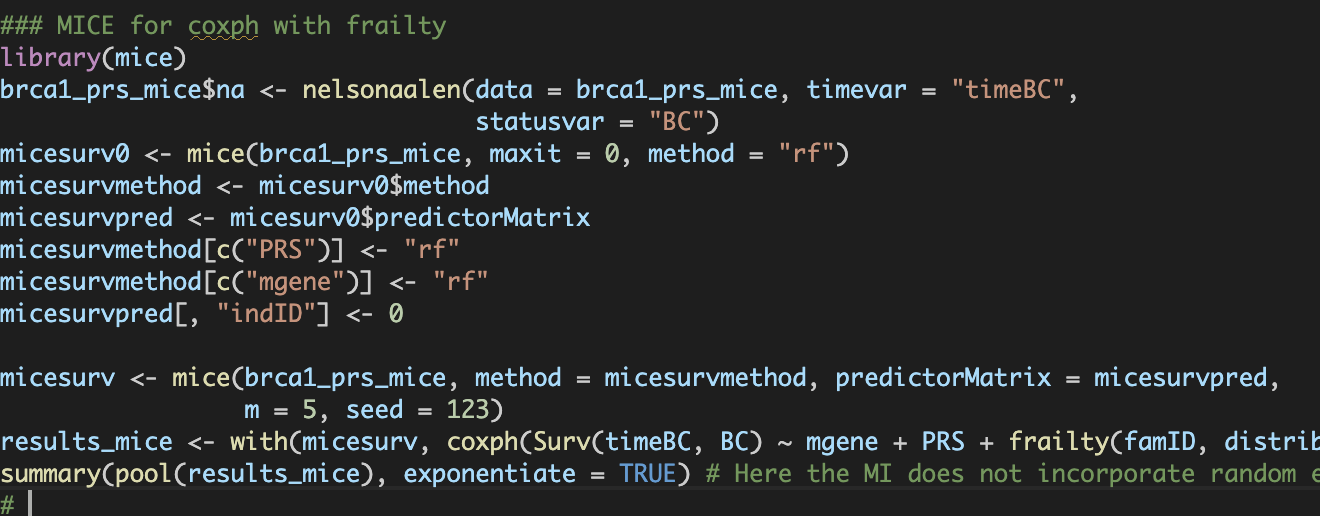
\includegraphics[width=0.5\linewidth]{Figuras/MICE in survival, fail to incorp frailty.png}
    \caption{MICE Code}\label{Fig:MICE no Frailty}
\end{figure}

Here I was trying to use random forest methods to impute both PRS and genotype, the performance of PRS seems good because the coefficient is close to the complete case analysis, but there is an inflation on the coefficient on genotype. 



%\newpage

%\section{References}
%\label{S.7}
%%
%% Following citation commands can be used in the body text:
%% Usage of \cite is as follows:
%%   \cite{key}          ==>>  [#]
%%   \cite[chap. 2]{key} ==>>  [#, chap. 2]
%%   \citet{key}         ==>>  Author [#]

%% References with bibTeX database:

%\bibliographystyle{model1-num-names}
%\bibliography{sample.bib}
%% Authors are advised to submit their bibtex database files. They are
%% requested to list a bibtex style file in the manuscript if they do
%% not want to use model1-num-names.bst.

%% References without bibTeX database:

%\begin{thebibliography}{00}

%% \bibitem must have the following form:
%%   \bibitem{key}...
%%

%\bibitem{}

%\end{thebibliography}


\end{document}

%%
%% End of file `elsarticle-template-1-num.tex'.